\chapter{Text detection}
\label{ch:detection}

The challenges presented in \autoref{sec:challenges} make it clear that a classical approach is unsuitable for our problem. As such, we direct our attention towards the modern, robust architectures of Convolutional Neural Networks (CNN) \citep{leCun_CNN}. In particular, we take inspiration from the great advances in object detection and we will treat text like a regular object which can be found anywhere in the image.

\Autoref{sec:faster_rcnn} introduces the first architecture we tested, the \FRCNN{} \citep{faster_rcnn}, as a mean of establishing a baseline. Then we explain how we produce data for training the architecture in \autoref{sec:detection_data} and how intermediate results drive us to more advanced data generation techniques. Then, \autoref{sec:ctpn} presents a more powerful architecure for text detection, the \emph{Connectionist Text Proposal Network}(\CTPN{}, \citet{ctpn}). \todo{Specify about detection results. First, we need to define what kind of results to present. Maybe just very short FRCNN vs CTPN on final constats => need to define benchmark.}


%========================================================================================

\section{Faster R-CNN}\label{sec:faster_rcnn}

	\begin{figure}
		\centering
		\includegraphics[width=0.85\linewidth]{fasterrcnn_diagram.pdf}
		\caption{The \FRCNN{} architecture (credit to \cite{detection_benchmark}) \label{fig:faster_rcnn}}
	\end{figure}

	The task of object detection builds upon that of image classification. Architectures based on region proposals (see \autoref{sec:related_detection}) can be seen as a two stage algorithm: the first part extracts possible object bounding boxes as a sub-image of the input, while the second one predicts the class associated with each candidate. It is of no surprise then that object detection greatly benefits from the super-human accuracy of deep neural networks \citep{superhuman_classif}. We chose to pair the \FRCNN{} detection architecture with the \RESNET{} feature extractor \citep{resnet}, since this has been proven as a good trade-off between detection accuracy and speed on the standard challenge of ILSCVR \citep{detection_benchmark}. In what follows we present the main building blocks of this architecture.

	%----------------------------------------------------------------------------------------

	\subsection{Feature extraction}\label{sec:resnet}
		In order to perform detection on an input image, we first need to extract representative high-level features from the raw pixel values. To this end, we employ the \RESNET{} convolutional architecture which has won many competitions in classification, detection and segmentation.

		The novelty of this approach\footnote{\todo{Should I dedicate a subsection to describe how (Conv) Neural Nets work?}} relies in forcing the network to learn a \emph{residual} mapping \(\mathcal{F}(\ve{x}) := \mathcal{H}(\ve{x}) - \ve{x}\), where \(\mathcal{H}(\ve{x})\) represents a desired mapping from input \(\ve{x}\), which is to be fit through a few stacked layers. This comes from the observation that the optimal function to be learnt could be closer to the identity mapping than to a zero mapping. Therefore, the new formulation eases the job of the optimiser since it only has to find perturbations around the identity mapping, rather than learn a completely new function.

		Moreover, in order to keep the number of parameters as small as possible and have reasonable training times for very deep architectures (101 layers), standard convolutions are replaced by bottleneck-blocks of convolutions (\autoref{fig:resnet} right). Such blocks are formed by concatenating a \(1 \times 1\) convolutional layer at each end of the \(3 \times 3\) layer. The ``prefix'' layer reduces the number of filters while the ``suffix'' one increases it back, thus reducing the computational cost of the heavier middle layer.

		\begin{figure}
			\centering
			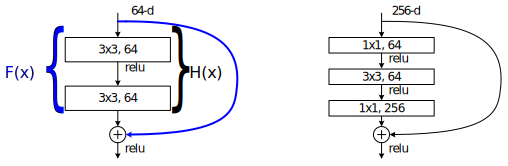
\includegraphics[width=0.85\linewidth]{resnet}
			\caption{ResNet blocks (\citet{resnet})
				\todo{Add \(\mathcal{H}(\ve{x})\) on the schema and small explanation.}
				\label{fig:resnet}
			}
		\end{figure}

		\todo{Show examples of extracted features for detection ? }

	%----------------------------------------------------------------------------------------

	\subsection{Region proposal network}\label{sec:frcnn_rpn}
		In order to bring the inference speed closer to real-time, \FRCNN{} improves on the bottleneck of previous approaches, namely the proposal of object candidates. Instead of relying on highly-engineered low-level features of super-pixels, the architecture reuses the convolutional feature map generated for the region classification step.

		This is achieved through another small, fully-convolutional network which is slided along the final layer of the feature map. The window at each location is projected into a lower dimensional feature that is used to predict \(k\) region bounds as well as \(k\) ``objectness'' scores. Each predicted region \(k_i\) is encoded as 4  coordinates \((x_1, y_1, x_2, y_2)_i\) that are \emph{relative} to a set of predefined boxes called \emph{anchors}. This mechanism allows the detection of multiple scales and aspect ratios in one pass through the network, thus avoiding the need of image pyramids and further reducing the computational cost.

		For training the RPN, the following loss function has to be minimised:
		\begin{equation}\label{eq:rpn_loss}
		L(\{p_i\}, \{t_i\}) = \frac{1}{N_{\cls}}\sum_i L_{\cls}(p_i, p^{*}_i) + \lambda\frac{1}{N_{\reg}}\sum_i  p^{*}_i L_{\reg}(t_i, t^{*}_i).
		\end{equation}
		It jointly minimised  the ``objectness'' classification  \(L_{\cls}\) for an anchor \(i\) in the minibatch and bounding box regression term \(L_{\reg}\), balanced by the hyperparameter \(\lambda\). The regression term is only taken into account for positive anchors (\(p^{*}_i = 1\)), which are those overlapping a ground-truth box with an Intersection-over-Union (IoU) ratio above threshold \(\tau = 0.7\).

	%----------------------------------------------------------------------------------------

	\subsection{Training}\label{sec:frcnn_train}
		The \FRCNN{} architecture can be trained end-to-end by jointly minimising the (weighted) sum of the RPN loss and the classification loss, as shown in \autoref{fig:faster_rcnn}. The forward pass generates box proposals that the classifier considers to be fixed for its training. This easy implementation ignores the gradients with regards to the coordinates of the proposal boxes, so it is only an approximation. However, its results are close to those obtained by alternating the training of the two networks, while being significantly faster.

		In order to speedup the training process, we make use of transfer learning and only fine-tune a detector that performs well on the ImageNet challenge. To this end, we replace the final softmax layer so that it only predicts among two classes: \texttt{text} or \texttt{background}.

		We hypothesize that the object / not-object distinction is easier to make for text detection in white background documents than it is for an ImageNet object. Therefore, we set hyperparameter \(\lambda = 2\) in order to give preference to the localisation loss. Moreover, in order to account for text's wide aspect ratio and relatively constant height in our documents, we generate similarly wide anchors (ratios \(\{2, 4, 6, 8, 10\}\)) with a limited set of scales (heights of \(\{50, 75, 100\}\)px). This further helps the box regression part to converge.

		We use the stochastic gradient descent (SGD) optimiser with momentum, on batches of 1 input image. Note, however, that a minibatch is formed of bounding boxes, so many candidates can be generated from a single input image and a set of anchors.


%========================================================================================


\section{Training data}\label{sec:detection_data}



%========================================================================================


\section{Connectionist Text Proposal Network}\label{sec:ctpn}


%----------------------------------------------------------------------------------------


%========================================================================================


\section{Results}\label{sec:detection_results}


%----------------------------------------------------------------------------------------
